\documentclass[11pt,a4paper]{article}
\newcommand{\intestazione}{Readout asimmetrico sul trimero ad anello}
% =====================================================================
%  Preambolo comune ai documenti sul dimero (serie "che cosa abbiamo fatto")
%  Incluso con % =====================================================================
%  Preambolo comune ai documenti sul dimero (serie "che cosa abbiamo fatto")
%  Incluso con % =====================================================================
%  Preambolo comune ai documenti sul dimero (serie "che cosa abbiamo fatto")
%  Incluso con \input{preambolo_dimero} subito dopo \documentclass.
% =====================================================================
\usepackage[T1]{fontenc}
\usepackage[utf8]{inputenc}
\usepackage[main=italian,provide=*]{babel}
\usepackage{amsmath,amssymb,mathtools}
\usepackage{graphicx}
\usepackage{booktabs}
\usepackage{colortbl}
\usepackage{xcolor}
\usepackage{geometry}
\usepackage{placeins}
\usepackage{caption}
\usepackage{enumitem}
\usepackage{fancyhdr}
\usepackage{needspace}
\usepackage{tikz}
\usetikzlibrary{arrows.meta,positioning,shapes.geometric,calc,fit,backgrounds}
\usepackage{hyperref}
\hypersetup{colorlinks=true,linkcolor=blu,citecolor=blu,urlcolor=blu}

\geometry{margin=2.5cm}

% --- colori coerenti con quelli delle figure (palette Okabe-Ito)
\definecolor{blu}{HTML}{0072B2}
\definecolor{arancio}{HTML}{E69F00}
\definecolor{verdes}{HTML}{009E73}
\definecolor{rossos}{HTML}{D55E00}
\definecolor{violas}{HTML}{CC79A7}
\definecolor{grigetto}{HTML}{E8E8E8}

\captionsetup{font=small,labelfont=bf,width=0.92\textwidth}

\pagestyle{fancy}
\fancyhf{}
\fancyhead[L]{\small\itshape\intestazione}
\fancyhead[R]{\small\thepage}
\renewcommand{\headrulewidth}{0.3pt}

% --- notazione
\newcommand{\ket}[1]{\lvert #1\rangle}
\newcommand{\bra}[1]{\langle #1 \rvert}
\newcommand{\media}[1]{\langle #1 \rangle}
\newcommand{\vs}[1]{\mathbf{s}_{#1}}

% --- riquadro "in una riga": il messaggio da portare a casa
\newcommand{\messaggio}[1]{%
  \begin{center}
  \begin{minipage}{0.93\textwidth}
  \setlength{\fboxsep}{9pt}%
  \colorbox{grigetto}{\begin{minipage}{\dimexpr\textwidth-2\fboxsep}
  \small\textbf{In una riga.}\enspace #1
  \end{minipage}}
  \end{minipage}
  \end{center}
}

% --- riquadro "come lo sappiamo": la verifica numerica dietro un'affermazione
\newcommand{\verifica}[1]{%
  \begin{center}
  \begin{minipage}{0.93\textwidth}
  \small\textcolor{verdes}{\rule{2.2em}{1.1pt}}\enspace
  \textcolor{verdes}{\textbf{Come lo sappiamo.}}\enspace #1
  \end{minipage}
  \end{center}
  \medskip
}
 subito dopo \documentclass.
% =====================================================================
\usepackage[T1]{fontenc}
\usepackage[utf8]{inputenc}
\usepackage[main=italian,provide=*]{babel}
\usepackage{amsmath,amssymb,mathtools}
\usepackage{graphicx}
\usepackage{booktabs}
\usepackage{colortbl}
\usepackage{xcolor}
\usepackage{geometry}
\usepackage{placeins}
\usepackage{caption}
\usepackage{enumitem}
\usepackage{fancyhdr}
\usepackage{needspace}
\usepackage{tikz}
\usetikzlibrary{arrows.meta,positioning,shapes.geometric,calc,fit,backgrounds}
\usepackage{hyperref}
\hypersetup{colorlinks=true,linkcolor=blu,citecolor=blu,urlcolor=blu}

\geometry{margin=2.5cm}

% --- colori coerenti con quelli delle figure (palette Okabe-Ito)
\definecolor{blu}{HTML}{0072B2}
\definecolor{arancio}{HTML}{E69F00}
\definecolor{verdes}{HTML}{009E73}
\definecolor{rossos}{HTML}{D55E00}
\definecolor{violas}{HTML}{CC79A7}
\definecolor{grigetto}{HTML}{E8E8E8}

\captionsetup{font=small,labelfont=bf,width=0.92\textwidth}

\pagestyle{fancy}
\fancyhf{}
\fancyhead[L]{\small\itshape\intestazione}
\fancyhead[R]{\small\thepage}
\renewcommand{\headrulewidth}{0.3pt}

% --- notazione
\newcommand{\ket}[1]{\lvert #1\rangle}
\newcommand{\bra}[1]{\langle #1 \rvert}
\newcommand{\media}[1]{\langle #1 \rangle}
\newcommand{\vs}[1]{\mathbf{s}_{#1}}

% --- riquadro "in una riga": il messaggio da portare a casa
\newcommand{\messaggio}[1]{%
  \begin{center}
  \begin{minipage}{0.93\textwidth}
  \setlength{\fboxsep}{9pt}%
  \colorbox{grigetto}{\begin{minipage}{\dimexpr\textwidth-2\fboxsep}
  \small\textbf{In una riga.}\enspace #1
  \end{minipage}}
  \end{minipage}
  \end{center}
}

% --- riquadro "come lo sappiamo": la verifica numerica dietro un'affermazione
\newcommand{\verifica}[1]{%
  \begin{center}
  \begin{minipage}{0.93\textwidth}
  \small\textcolor{verdes}{\rule{2.2em}{1.1pt}}\enspace
  \textcolor{verdes}{\textbf{Come lo sappiamo.}}\enspace #1
  \end{minipage}
  \end{center}
  \medskip
}
 subito dopo \documentclass.
% =====================================================================
\usepackage[T1]{fontenc}
\usepackage[utf8]{inputenc}
\usepackage[main=italian,provide=*]{babel}
\usepackage{amsmath,amssymb,mathtools}
\usepackage{graphicx}
\usepackage{booktabs}
\usepackage{colortbl}
\usepackage{xcolor}
\usepackage{geometry}
\usepackage{placeins}
\usepackage{caption}
\usepackage{enumitem}
\usepackage{fancyhdr}
\usepackage{needspace}
\usepackage{tikz}
\usetikzlibrary{arrows.meta,positioning,shapes.geometric,calc,fit,backgrounds}
\usepackage{hyperref}
\hypersetup{colorlinks=true,linkcolor=blu,citecolor=blu,urlcolor=blu}

\geometry{margin=2.5cm}

% --- colori coerenti con quelli delle figure (palette Okabe-Ito)
\definecolor{blu}{HTML}{0072B2}
\definecolor{arancio}{HTML}{E69F00}
\definecolor{verdes}{HTML}{009E73}
\definecolor{rossos}{HTML}{D55E00}
\definecolor{violas}{HTML}{CC79A7}
\definecolor{grigetto}{HTML}{E8E8E8}

\captionsetup{font=small,labelfont=bf,width=0.92\textwidth}

\pagestyle{fancy}
\fancyhf{}
\fancyhead[L]{\small\itshape\intestazione}
\fancyhead[R]{\small\thepage}
\renewcommand{\headrulewidth}{0.3pt}

% --- notazione
\newcommand{\ket}[1]{\lvert #1\rangle}
\newcommand{\bra}[1]{\langle #1 \rvert}
\newcommand{\media}[1]{\langle #1 \rangle}
\newcommand{\vs}[1]{\mathbf{s}_{#1}}

% --- riquadro "in una riga": il messaggio da portare a casa
\newcommand{\messaggio}[1]{%
  \begin{center}
  \begin{minipage}{0.93\textwidth}
  \setlength{\fboxsep}{9pt}%
  \colorbox{grigetto}{\begin{minipage}{\dimexpr\textwidth-2\fboxsep}
  \small\textbf{In una riga.}\enspace #1
  \end{minipage}}
  \end{minipage}
  \end{center}
}

% --- riquadro "come lo sappiamo": la verifica numerica dietro un'affermazione
\newcommand{\verifica}[1]{%
  \begin{center}
  \begin{minipage}{0.93\textwidth}
  \small\textcolor{verdes}{\rule{2.2em}{1.1pt}}\enspace
  \textcolor{verdes}{\textbf{Come lo sappiamo.}}\enspace #1
  \end{minipage}
  \end{center}
  \medskip
}

\providecommand{\Tr}{\operatorname{Tr}}

\title{\bfseries Readout asimmetrico sul trimero ad anello\\[2pt]
\large Resoconto definitivo: teoria, verifica, stress test}
\author{Samuele Schiavi \\ \small Tesi triennale in Fisica, Università di Parma
--- Relatore: Prof.\ Alessandro Chiesa}
\date{}

\begin{document}
\maketitle
\thispagestyle{fancy}

\noindent\textbf{File di codice}:
\begin{itemize}[nosep,leftmargin=1.3em]
  \item \texttt{correlatori\_readout\_asimmetrico\_trimero\_anello.py}
  \item \texttt{validate\_correlatori\_readout\_asimmetrico\_trimero\_anello.py}
\end{itemize}
\noindent Punto di
lavoro: Scenario A ($J{=}1,J'{=}0.4,b{=}b_c{=}2.4,D{=}0.15$), correlatore $C_{21}^{xx}(t{=}2)$,
baseline $N^*=3$ (Stadio 4). Mirror diretto di
\texttt{correlatori\_readout\_asimmetrico.py} (dimero).

\tableofcontents

% =====================================================================
\section{Obiettivo}
% =====================================================================

Estensione facoltativa già chiusa sul dimero: verificare se $N^*=\arg\max_N|C(N)|$ resta
invariato quando l'errore di lettura smette di essere simmetrico ($p_{01}=p_{10}=p$) e diventa
$p_{01}\neq p_{10}$, come è tipicamente il caso su hardware reale (rilassamento $T_1$ durante la
misura rende $p_{10}>p_{01}$).

\messaggio{A differenza dell'estensione 1 (VQE noise-aware), qui non è emerso nulla di nuovo
rispetto al dimero: nessun ostacolo concettuale, nessun comportamento anomalo. L'unico punto
richiedeva attenzione --- la diversa convenzione dei qubit --- ed è stato verificato
esplicitamente prima di scrivere il resto del codice.}

% =====================================================================
\section{Perché non ci si aspettava (e non si è trovato) nulla di nuovo}
% =====================================================================

Verificato nel documento dei punti di lavoro, prima ancora di scrivere questo codice: il circuito
dei correlatori dell'anello (4 qubit: 3 di registro + 1 ancilla) misura, esattamente come sul
dimero, \textbf{un solo bit classico, sempre e solo l'ancilla}
(\texttt{qc.measure(ANCILLA, 0)} nella versione base). La correzione di readout asimmetrico si
applica a quella singola misura --- una proprietà del \emph{numero di bit misurati}, non del
numero di qubit di registro nel circuito coerente che precede la misura. Il numero maggiore di
qubit di registro dell'anello (3 contro 2) non introduce quindi nessuna considerazione nuova.

% =====================================================================
\section{Un dettaglio verificato esplicitamente: la convenzione dei qubit}
% =====================================================================

Sul dimero l'ancilla è il qubit 0: con \texttt{measure\_all()} su un registro a 3 qubit, il suo
bit è l'\textbf{ultimo} carattere della stringa di misura (\texttt{bitstr[-1]}, convenzione
little-endian di Qiskit). Sull'anello l'ancilla è il qubit 3 (convenzione ereditata da Parte 1):
con \texttt{measure\_all()} su 4 qubit, il suo bit è invece il \textbf{primo} carattere.

\verifica{Circuito di controllo: $X$ applicato solo all'ancilla, registro nello stato $\ket{000}$,
100 shot. Risultato: \texttt{\{'1000': 100\}} --- il bit dell'ancilla è la prima cifra della
stringa, non l'ultima. Verificato \emph{prima} di scrivere il cross-check Monte Carlo, per non
riprodurre in silenzio un errore di indicizzazione ereditato dal dimero.}

% =====================================================================
\section{Teoria: stessa formula del dimero}
% =====================================================================

Nessuna nuova derivazione necessaria --- la formula generale del readout asimmetrico è una
proprietà della singola misura, indipendente dal sistema fisico a monte:
$$\langle Z\rangle_\text{readout} = \alpha\langle Z\rangle_\text{ideale} + \beta,
\qquad \alpha = 1-p_{01}-p_{10},\ \ \beta = p_{10}-p_{01},$$
che per il correlatore complesso diventa $C_\text{readout}(N) = \alpha\,C_\text{ideale}(N) +
\beta(1+i)$ --- non garantita a priori preservare l'invarianza di $N^*$ (somma e modulo non
commutano), esattamente come sul dimero.

% =====================================================================
\section{Metodologia: formula analitica + cross-check Monte Carlo (shot veri)}
% =====================================================================

Allineata allo standard ora in uso sul dimero (readout genuinamente campionato, non solo formula
analitica): ogni punto è verificato su \textbf{due percorsi indipendenti}.
\begin{itemize}[nosep]
  \item \textbf{Analitico}: formula sopra applicata a $\langle Z\rangle_\text{ideale}$ dalla
  simulazione a operatore densità (esatta, nessun rumore statistico).
  \item \textbf{Monte Carlo}: \texttt{ReadoutError} \emph{vero} (matrice di confusione
  asimmetrica) agganciato al \texttt{NoiseModel}, misura a $2\times10^5$ shot, nessuna formula.
\end{itemize}

% =====================================================================
\section{Risultato 1: limite di rumore nullo e limite simmetrico}
% =====================================================================

\begin{table}[htbp]
\centering
\caption{Controlli di limite, prima di guardare il caso genuinamente asimmetrico.}
\begin{tabular}{p{5.7cm}p{3.7cm}p{4.3cm}}
\toprule
Controllo & Atteso & Trovato \\
\midrule
$p_{01}=p_{10}=0$ vs ramo originale ($p_\text{readout}=0$) & coincidenza esatta & $|$diff$|=0$ (precisione macchina) \\
$p_{01}=p_{10}=2.3\times10^{-2}$ & $N^*=3$ & $N^*=3$, $|C(N^*)|=0.5048$ \\
\bottomrule
\end{tabular}
\end{table}

Entrambi superati: il ramo asimmetrico degenera esattamente in quello simmetrico/originale nei
rispettivi limiti, e riproduce il baseline $N^*=3$ già noto dallo Stadio 4.

% =====================================================================
\section{Risultato 2: split illustrativo e cross-check Monte Carlo}
% =====================================================================

Split illustrativo (non una calibrazione reale citabile per \texttt{ibm\_torino} specificamente
--- stessa scelta già motivata sul dimero): rapporto $p_{10}/p_{01}=3\times$, stessa media
$p_\text{readout}=2.3\times10^{-2}$ già in uso ($p_{01}=0.0115$, $p_{10}=0.0345$).

\begin{figure}[htbp]
\centering
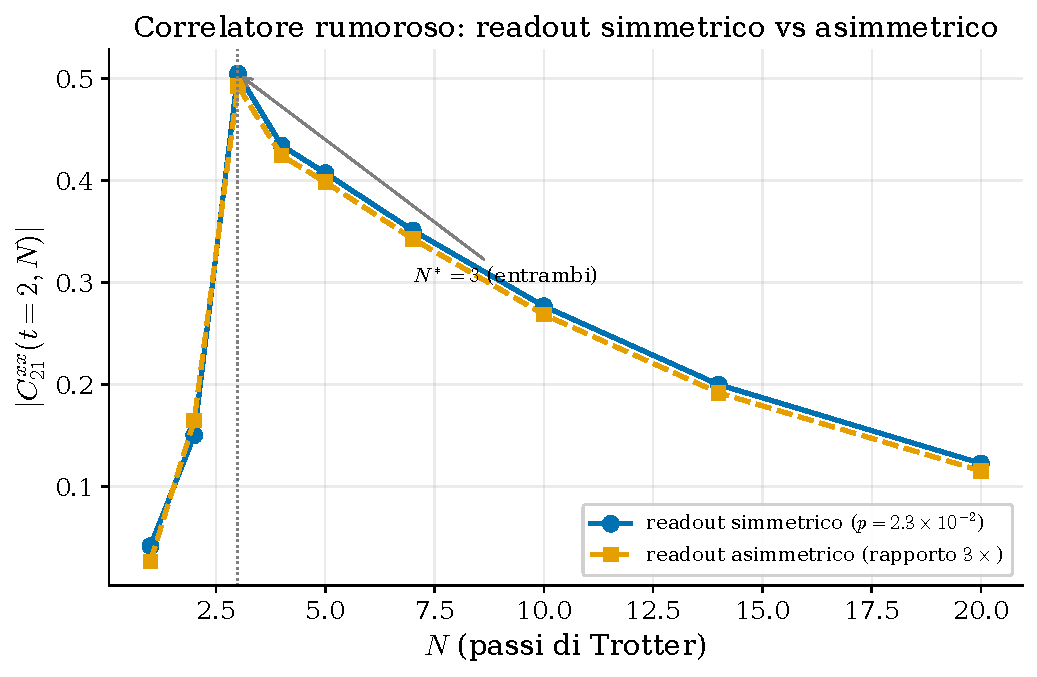
\includegraphics[width=0.78\textwidth]{figure/fig_correlatore_readout_asimmetrico_trimero_anello.pdf}
\caption{Modulo del correlatore $|C_{21}^{xx}(t{=}2,N)|$, readout simmetrico contro asimmetrico
(rapporto $3\times$). $N^*=3$ in entrambi i casi; lo scostamento è piccolo e monotono, ben lontano
dallo spostare il massimo.}
\end{figure}

\begin{table}[htbp]
\centering
\caption{Cross-check Monte Carlo, split illustrativo ($2\times10^5$ shot).}
\begin{tabular}{lccc}
\toprule
$N$ & Analitico & Monte Carlo & $|$diff$|$ \\
\midrule
3 & $-0.448046+0.204565i$ & $-0.446280+0.207010i$ & $3.02\times10^{-3}$ \\
5 & $-0.339490+0.208655i$ & $-0.336380+0.211240i$ & $4.04\times10^{-3}$ \\
\bottomrule
\end{tabular}
\end{table}

Scostamento coerente con l'errore statistico atteso per $2\times10^5$ shot
($\sim1/\sqrt{2\times10^5}\approx2.2\times10^{-3}$ per componente) --- i due percorsi di calcolo,
completamente indipendenti, si confermano a vicenda.

$N^*$ (asimmetrico) $=3$, $|C(N^*)|=0.4925$ --- invariato rispetto al caso simmetrico
($N^*=3$, $|C(N^*)|=0.5048$).

% =====================================================================
\section{Risultato 3: stress test fino a $50\times$}
% =====================================================================

\begin{figure}[htbp]
\centering
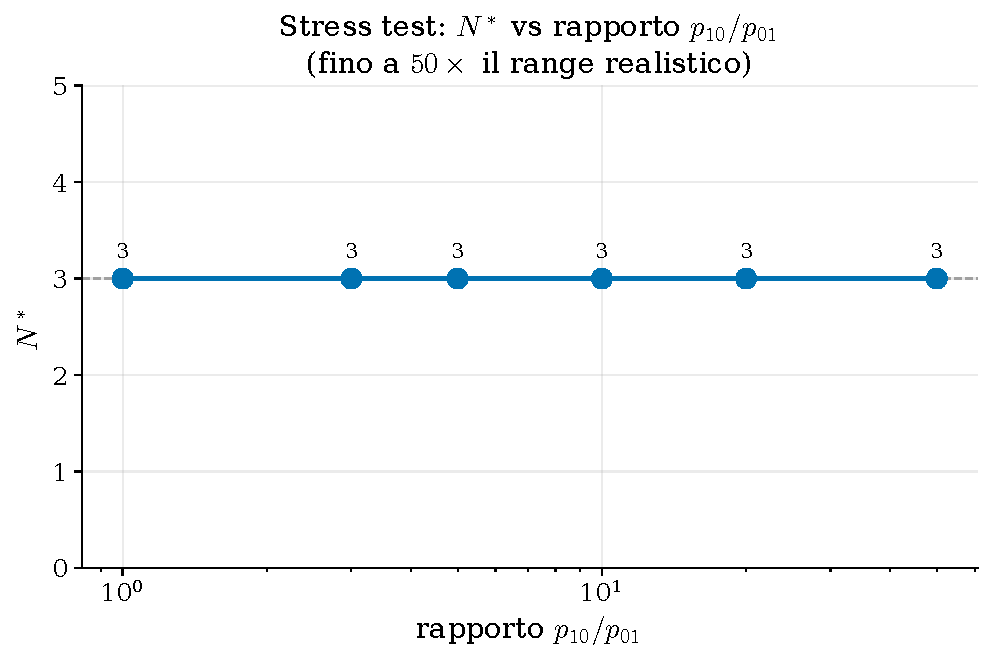
\includegraphics[width=0.72\textwidth]{figure/fig_stress_readout_asimmetrico_trimero_anello.pdf}
\caption{$N^*$ in funzione del rapporto $p_{10}/p_{01}$, da $1\times$ (simmetrico) a $50\times$
--- ben oltre il range realistico osservato su hardware IBM (tipicamente $2$--$3.5\times$).
$N^*=3$ su tutti i punti testati.}
\end{figure}

\begin{table}[htbp]
\centering
\caption{Stress test: $N^*$ per rapporti $p_{10}/p_{01}$ crescenti, stessa media
$p_\text{readout}=2.3\times10^{-2}$.}
\begin{tabular}{lccc}
\toprule
Rapporto & $p_{01}$ & $p_{10}$ & $N^*$ ($|C(N^*)|$) \\
\midrule
$1\times$ & 0.0230 & 0.0230 & 3 (0.5048) \\
$3\times$ & 0.0115 & 0.0345 & 3 (0.4925) \\
$5\times$ & 0.0077 & 0.0383 & 3 (0.4889) \\
$10\times$ & 0.0042 & 0.0418 & 3 (0.4857) \\
$20\times$ & 0.0022 & 0.0438 & 3 (0.4840) \\
$50\times$ & 0.0009 & 0.0451 & 3 (0.4829) \\
\bottomrule
\end{tabular}
\end{table}

$N^*=3$ invariato su tutti i sei rapporti testati, incluso il punto più estremo ($50\times$, ben
oltre qualunque split osservato su hardware reale). Stesso esito qualitativo del dimero.

% =====================================================================
\section{Confronto con il dimero}
% =====================================================================

\begin{table}[htbp]
\centering
\caption{Riepilogo comparativo, estensione readout asimmetrico.}
\begin{tabular}{lcc}
\toprule
& Dimero & Trimero ad anello \\
\midrule
Qubit di registro & 2 & 3 \\
Qubit totali nel circuito correlatori & 3 & 4 \\
Qubit misurati per il readout & 1 (ancilla) & 1 (ancilla) \\
Convenzione ancilla & qubit 0 (ultimo bit) & qubit 3 (primo bit) \\
$N^*$ simmetrico (baseline) & 2 (dopo correzione correlatore) & 3 \\
$N^*$ split illustrativo $3\times$ & invariato & invariato \\
Stress test massimo & $50\times$ & $50\times$ \\
Esito stress test & invariato & invariato \\
Metodologia & analitico + Monte Carlo & analitico + Monte Carlo \\
\bottomrule
\end{tabular}
\end{table}

% =====================================================================
\section{Conclusioni}
% =====================================================================

Estensione chiusa senza sorprese, a differenza dell'estensione 1: nessun ostacolo concettuale
confermato (il numero maggiore di qubit di registro non tocca la correzione, che si applica a una
singola misura), nessun comportamento anomalo emerso. L'unico punto che richiedeva attenzione ---
la diversa convenzione dei qubit dell'ancilla --- è stato identificato e verificato esplicitamente
prima di scrivere il codice, non scoperto a posteriori da un risultato sbagliato.

\subsection*{Sintesi in una riga}
$N^*=3$ non si sposta per readout asimmetrico, verificato su formula analitica e cross-check
Monte Carlo indipendente, fino a rapporti $50\times$ oltre il range realistico --- stesso esito
qualitativo del dimero, nessuna complicazione dal registro a 3 qubit.

\subsection*{File prodotti}
\begin{itemize}[nosep,leftmargin=1.3em]
  \item \texttt{correlatori\_readout\_asimmetrico\_trimero\_anello.py} (formula, cross-check
  Monte Carlo, stress test)
  \item \texttt{validate\_correlatori\_readout\_asimmetrico\_trimero\_anello.py} (6 controlli)
  \item questo documento e le sue 2 figure
\end{itemize}
\noindent Aggiornamento in \texttt{log\_decisioni.md}, \texttt{scheda\_progetto\_tesi.md}.

\end{document}
